\chapter{ Computational methods }
\label{chap3}


Cosmology tries to explain the evolution of structures 
from its first stages to the actual epoch, which leads to
the current large scale structure. 
Thus, it is necessary to study the evolution of the matter content 
of the Universe under the influence of gravity. To solve this,
the Boltzmann equation (BE) could be used since it allows to predict the statistical
behavior of a system that is not in equilibrium. Hence, a probability density 
distribution for the system would be obtained from solving the BE.
Though, this system is so complex that is necessary to make a different approach
\cite{bosch}. 
In this direction, it possible to assume an initial density field
as one specific realization of the probability density distribution, i.e. 
a specific particle distribution that would trace the initial density field. 
Now, using this initial particle distribution, the evolution of the system
would be obtained finding the interaction among particles.  
Thus, due to the big amount of interacting particles necessary to simulate
the system, computational resources appear as a necessary tool to tackle such problems. 
Hence, numerical approximations 
must be developed to find, for every time, step all the properties needed to describe 
the system, even when particles studied have masses with an order of magnitude of several 
stellar masses. 

In cosmological simulations of structure formation, a key component to consider
is dark matter, because dark matter dominates the gravitational
interaction, not only because of its amount compared to
baryonic matter but also because it only interacts in this way.
It is mostly because of this that the Universe has a sponge-like
structure at large scales \cite{kyplin1}. 

Defining as total density, the sum of baryonic and dark matter,
it can be given an argument to ignore baryonic matter in simulations: 
dark matter would contribute with around $80\%$ of all 
the density content. Hence, the assumption that the large scale
structure formation is determined by dark matter is plausible \cite{Longair}.

This chapter is divided in five sections, the first one
corresponds to the methods used in cosmological simulations to
calculate the gravitational evolution of the system \cite{Klypin1},\cite{Klypin2}
and \cite{Klypin3}. The second
one contains different criteria selection to detect a dark matter
halo in simulations. The third section explains how to obtain 
a density field from a cosmological simulation. The fourth and fifth 
sections are dedicated to explain how to build different statistical 
measures of clustering, the correlation function in real space and 
the power spectrum in fourier space.

\begin{comment} 
Detailed description can be found in \cite{Djeong}, \cite{Longair}, \cite{tree}, \cite{Klypin}, \cite{Klypin2},\cite{Klypin3}, \cite{Jing}, \cite{Mont}.
\end{comment}

%&&&&&&&&&&&&&&&&&&&&&&&&&&&&&&&&&&&&&&&&&&&&&&&&&&&&&&&&&&&&&&&&&&&&&&&&&&&&&&&&&&&&&&&&&&&&&&&&&&&&&&&&&&&&&&&&&&&&&&
\section{ Numerical methods }
%&&&&&&&&&&&&&&&&&&&&&&&&&&&&&&&&&&&&&&&&&&&&&&&&&&&&&&&&&&&&&&&&&&&&&&&&&&&&&&&&&&&&&&&&&&&&&&&&&&&&&&&&&&&&&&&&&&&&&&


To study the formation of the large scale structure, simulations of dark matter
are performed, i.e., a cosmological box where dark matter particles interact gravitationally. 
In such cases it is necessary to suppose initial conditions,
an initial configuration of the Universe, i.e., an initial density field
or an initial shape for the power spectrum. 
Furthermore, two important parameters for this cosmological simulations are the box 
size $L$ and the number of dark matter particles $N_p^3$ that would trace the initial
density field, among others. 

The gravitational interaction calculation of such a big number of particles
could, in principle, be calculated through direct sum of forces. This first
attempt is not very efficient, or even, it is not possible to perform,
since the computing time or the computational resources would be very 
big to be viable \cite{tree}. This is the reason for approximate methods 
to appear as a possible solution that would require more reasonable computing times.

A main objective in a simulation is the study the formation process and
further interactions that are produced among halos and vacuum regions that conform
the sponge-like structure of the Universe. Next, two numerical 
methods used for cosmological simulations, are going to be briefly exposed:

\begin{enumerate}
\item \textbf{Particle Mesh (PM)}

In this method a grid is created over the particle array,
i.e., the cosmological box that contains the particles is divided in 
cells of the same size. 
But, to show the basics of this method, a 2D example is explained, 
as shown in the figure \ref{PM}. In this case, the particles closer
to a vertex, each representing a specific cell, are assigned to this one \cite{tree}.
Then, an approximated density field is calculated using 
the mass per cell divided by its area. 
Other way to calculate the density field is cloud in cell, later explained
in more detail, where particles are considered constant density cubes causing
that a single particle contributes to different cells.
Now, using the density field and the Poisson equation, it is possible to calculate 
the gravitational potential in every grid vertex.

This method reduces considerably the computing time 
since its of the order of O($N+M\log M$) with $N$ being the number of particles
and $M$ the number of vertex. Although, the lack of resolution in the regions that are
more dense makes this method insufficient to respond for the physical situation.
Furthermore, it does not give account for a complex geometry or systems
higly correlated. A step forward in this direction is $P^3M$ that uses for smaller scales finer calculations of the potential performing a particle particle calculation. 

%**********************************************************************************************************************
\begin{figure}[htbp]
       \centering
               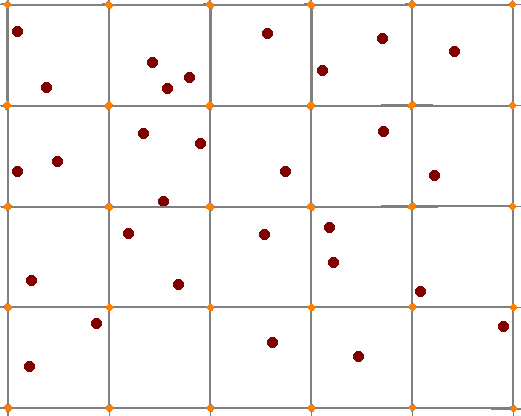
\includegraphics[width=0.35\textwidth]{Images/chapter3/MG.png}
       \caption{\small Particle mesh method. Every vertex of the grid gets 
       properties calculated from the closer particles.}
       \label{PM}
 \end{figure}
%**********************************************************************************************************************


\item \textbf{Tree method}


To illustrate this method let us consider a 2D particle array. 
In this case, the cosmological box is represented by a square.
It is divided in cells of the same area where
each particle is assigned to the cell where it falls in \cite{tree}. 
If the number of particles is superior to one, subdivisions 
of the cell are performed. Again, if the number of particles 
per subcells is superior to one, subdivisions are made. This
process is repeated until for every cell there is at most
one particle. 
This subdivision is used to create a tree structure, this consists
in a root, i.e., all the square area and the branches that are 
created with each subdivision performed. This works as a map
of the disposition of the particles in the square array. 
The particles are numbered from the upper left of the square 
until reaching the lower right of the square. All particles in the
same cell must numered before continuing with the next cell, as
shown in the figure \ref{tree}. 

When the gravitational calculation is performed, the contribution 
to the force exerted over a particle due to the more distant ones
is much lower than with the nearer ones. Thus, the far ones can be 
approximated as a pseudoparticle with mass $M$ and with a position
$r_{CM}=\sum_im_ir_i/M$. The next expression is taken as a selection 
criteria \cite{tree} : 

\begin{equation}
s/q\leq \theta,
\label{sq}
\end{equation}

where $s$ is the cell size with wich the particle of interest is interacting 
with, $d$ the distance between the cell and the particle,
and $\theta$ is a tolerance value to define. 
For each particle, the gravitational interaction with the other particles 
or pseudoparticles is calculated according to the criteria \ref{sq}. 
If the condition is satisfied the gravitational interaction 
is calculated directly with the pseudoparticle (or particle) as shown in figure \ref{tree}. 
If the relation is not satisfied, it is necessary to divide the cell into 
subcells, and that way successively until the condition is satisfied, or only one 
particle is present per subcell. Thus, the direct calculation is avoided for far
objects, without avoiding the calculation for the nearer ones. 
Therefore, the computing time is reduced from $O(N^2)$ to $O(N\log(N))$, i.e., it is cheaper
computationally. 

%**********************************************************************************************************************
\begin{figure}[htbp]
       \centering
               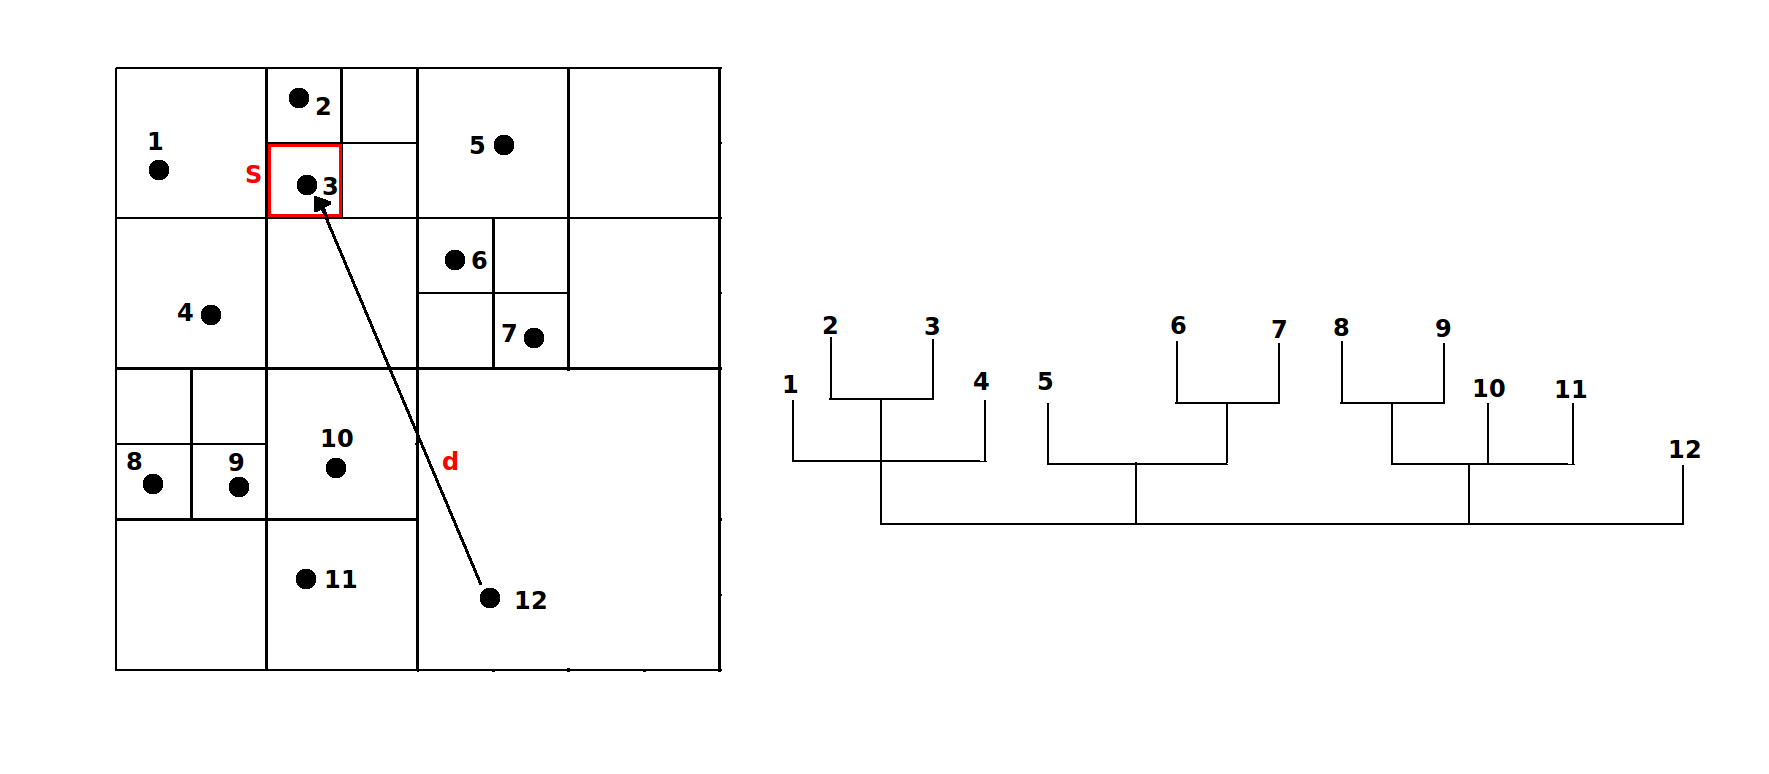
\includegraphics[width=1.0\textwidth]{Images/chapter3/treecode.png}
       \caption{\small In the left panel is shown the array of the particles and the subdivisions performed until the criteria \label{sq} is satisfied. In the right one, the tree found for such distribution is shown.}
       \label{tree}
 \end{figure}
%**********************************************************************************************************************

\end{enumerate}

There are many methods that are hibrid of the two exposed. For example, 
$P^3M$ that was already mentioned. All of them have both, advantages and disadvantages,
that must be evaluated according to the needs of the simulation. 

\

%&&&&&&&&&&&&&&&&&&&&&&&&&&&&&&&&&&&&&&&&&&&&&&&&&&&&&&&&&&&&&&&&&&&&&&&&&&&&&&&&&&&&&&&&&&&&&&&&&&&&&&&&&&&&&&&&&&&&&&
\section{ Halo selection }
%&&&&&&&&&&&&&&&&&&&&&&&&&&&&&&&&&&&&&&&&&&&&&&&&&&&&&&&&&&&&&&&&&&&&&&&&&&&&&&&&&&&&&&&&&&&&&&&&&&&&&&&&&&&&&&&&&&&&&&

As a result of the dark matter particle interactions, perturbations 
grow enough to form bound objects that we will assume are in virial equilibrium,
these are known as dark matter halos and satisfy the relation $E_k=-V/2$ where
$E_k$ is the kinetic energy and $V$ is the potential energy. 
They are responsible for the potential wells that causes baryonic matter 
to fall in, forming finally the galaxies we observe today, i.e., dark
matter halos host galaxies. 

A main result of a cosmological simulation are the dark matter halos 
catalogue, which we are going to work with, that contains halo properties such
position, velocity, mass and radius. Therefore, a key step is to identify 
halos from a cosmological simulation, the methods generally use to acomplish such 
task are FOF and BDM \footnote{\url{https://www.cosmosim.org/cms/simulations/halo-finders/}}.

\begin{enumerate}

%######################################################################################################################
%\subsection{ Friends of friends }
%######################################################################################################################

\item \textbf{Friend of Friends (FOF)} 

To identify if a particle group lies in a dark matter halo, i.e., particles 
are bound, a length is defined such that all the particles with their distances 
lower than this length are part of the same group. This treshold is called linking length. 
A condition is imposed, groups can not intersect among them, hence a particle can only belong 
to a specific group. 

%**********************************************************************************************************************
\begin{figure}[htbp]
       \centering
               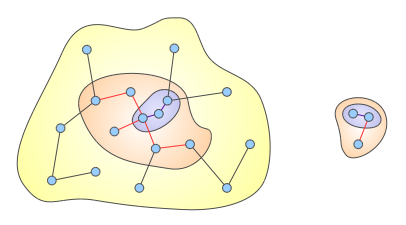
\includegraphics[width=0.5\textwidth]{Images/chapter3/FOFgroups.png}
       \caption{\small  \href{https://www.cosmosim.org/}{Image taken from Cosmosim database.} }
       \label{tree}
 \end{figure}
%**********************************************************************************************************************


But there is a problem with this approach. Even when there is 
a little amount of particles in common between two groups, some sort of small 
``bridge`` that unites both of them, they are selected as one group, not two,
as would be expected. This method also allows to define substructures, therefore using
different linking lengths, groups inside groups would be obtained, the bigger ones
would host the smaller ones. 

%######################################################################################################################
%\subsection{ Bound density maximum }
%######################################################################################################################

\item \textbf{Bound Density Maximun(BDM)}

This method, to select dark matter halos, uses local maximum densities
in the matter distribution of the simulation.  
The local maximum densities allows to define a spherical cut, the dark matter halo, 
and the particles that fall inside belongs to that specific halo \footnote{\url{https://www.cosmosim.org/cms/simulations/halo-finders/}}. 
Particles with a velocity equal or bigger to the scape velocity are 
not included in the halo. 
Contrary to FOF method, halos can overlap while the center of mass of one halo 
does not fall into other halo. Nevertheless, if the center of mass of one halo
falls in the virial radius of other one, the first one is considered a subhalo of the last
one. The standard overdensity limit of the halos is $\sim 360$ $\rho_{back}$ where $\rho_{back}$
is the background density. 

\end{enumerate}

%&&&&&&&&&&&&&&&&&&&&&&&&&&&&&&&&&&&&&&&&&&&&&&&&&&&&&&&&&&&&&&&&&&&&&&&&&&&&&&&&&&&&&&&&&&&&&&&&&&&&&&&&&&&&&&&&&&&&&&
\section{Density field in a cosmological simulation}
%&&&&&&&&&&&&&&&&&&&&&&&&&&&&&&&&&&&&&&&&&&&&&&&&&&&&&&&&&&&&&&&&&&&&&&&&&&&&&&&&&&&&&&&&&&&&&&&&&&&&&&&&&&&&&&&&&&&&&&

To construct a good approximation of the real density field from a cosmological simulation, 
a sampling of the continuous density field in a regular grid of size $N^3$ is 
performed, the subdivisions created are called cells. Hence, an assignment of the 
particle charge, i.e. particle mass, to the grid must be done. To obtain a more realistic 
density field approximation the grid points can be increased also disminishing problems 
due to numerical effects but it is more expensive computationally. Furthermore, the number 
of particles in a simulation is a restriction to the maximum value that $N$ can have, 
it can not exceed $\sqrt[3]{N_p}$, there would not be enough particles to map correctly 
the density field per cell. A size grid around the value mentioned would optimal in 
the sense that the particle mean per cell would be one, hence a Poisson distribution 
would be followed. But the sampling made from the particle distribution is not a 
mere sampling but a sampling convolved with a window function (the way a particle 
mass is distributed in the grid), i.e., the window function $W(\textbf{x})$ that is used affects 
the density field calculated \cite{bosch}. 

Since the particles are located in a specific position it can be assured that
the particle number density is: 

\[n_0(\textbf{x}) = \sum_{i=1}^{N_{p}} \delta^D ( \textbf{x} - \textbf{x}_i ),\]

where $\textbf{x}_i$ the position of the $i$-th particle. The window function 
quantifies how much of the particle number density is distributed to a grid point 
separated by $\textbf{x}$, hence the sample particle number density can expressed as: 

\[n(\textbf{x}_p) = \int_V d^3 x' n_0(\textbf{x'}) W(\textbf{x}_p-\textbf{x'}).\]

Similarly, the sampled density contrast defined as $\delta^s(\textbf{x})=n(\textbf{x}_p)/\bar{n}-1$ 
can be found using the convolution of the real density contrast and the window function: 

\begin{equation}
\delta^s(\textbf{x}) = [\delta*W](\textbf{x}),
\label{df_conv}
\end{equation}

its fourier transformation is simply the product of the fourier transformation of the real 
density contrast and the window function: 

\begin{equation}
\delta^s(\textbf{k}) = \delta(\textbf{k})W(\textbf{k}),
\label{df_four}
\end{equation}

thus, the real density contrast can be obtained dividing the sampled density contrast with
the window function used. 

\

The procedure of convolving with a window function can be seen in a different way, if a 
point spreading or cloud shape function $S(x')$, being $x'$ the distance from the particle
position $x_i$, is carried by each particle then the charge assigned to the grid point $x_p$ 
is given by the overlap of the shape function within the cubic cell $p$:

\[W(x)=\int \Pi \left(\frac{x'}{H} \right) S(x'-x)dx', \]

where $\Pi(x)$ is the top hot function and $H=L/N$ is the size of a cell. 

There are 3 commonly used schemes for the mass assignment, nearest grid point, cloud
in cell and triangular shaped cloud \cite{hockney}. For each case we are going to 
consider a one dimensional window function. The sencond and third are first 
and second order distribution schemes respectively, hence each of them is a better 
approximation than the previous one. 

\begin{enumerate}

\item \textbf{ Nearest grid point (NGP):} The first scheme considers that the particle mass is 
assigned to the cell where the particle falls, each cell is centered 
in a grid point, therefore the particle is assigned to the nearest grid point. 
Let us see this in more detail using two different interpretations \cite{hockney}. 
If a cloud shape interpretation is used, the particle 
shape would be a Dirac delta function that would be assigned to the specific cell 
where particle falls in as shown in the left figure of \ref{NGP}. Other interpretation 
could be considered, where the window function would be a top hat function centered in the particle. 
In this scenario, the value assigned to grid point would the one that top hat function 
would get when is evaluated in that grid point as shown in right figure of \ref{NGP}. 

\begin{eqnarray*}
 W_{NGP}(x)  =  \Pi \left( \frac{x}{H} \right) & \equiv & \frac{1}{H}\Pi\left(\frac{x}{H}\right) *\delta \left(\frac{x}{H}\right) \\ 
&  = &\frac{1}{H}\Pi\left(\frac{x}{H}\right)*S\left(\frac{x}{H}\right)
\end{eqnarray*}

This window function in the fourier space is

\[ W_{NGP}(k)= sinc\left(\frac{\pi k}{2k_N} \right)\]

where $k_N$ is the Nyquist frequency.

\

%**********************************************************************************************************************
\begin{figure}[htbp]
       \centering
               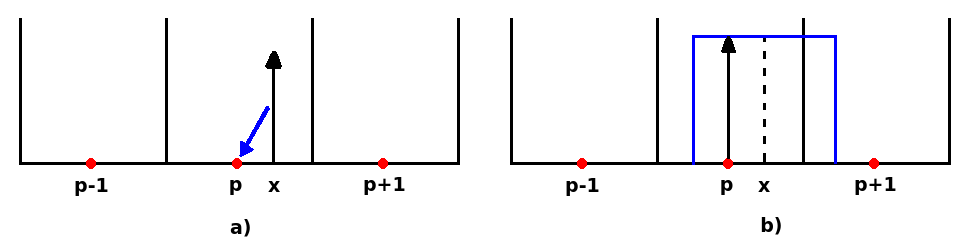
\includegraphics[width=0.8\textwidth]{Images/chapter3/NGP.png}
       \caption{\small Left: the cloud shape interpretation where the Dirac function
       is assigned to the particle grid. Right: it shows the window function interpretation
       where the top hat function evaluated in the grid point would give the mass assigned to it. 
       $x$ is the position of the particle and the indexes $p-1$, $p$ and $p+1$ are contiguous cells. }
       \label{NGP}
 \end{figure}
%**********************************************************************************************************************

\item \textbf{ Cloud in cell (CIC): } This scheme assumes that the mass of a specific particle 
assigned to a grid point is given by the overlap of a cell with a size H centered in 
the particle with the cell centered any the grid point. Then, the particle not only 
contributes to the cell where it falls in, but also to some of the 26 neighbour cells. 
This explanation is shown in the left figure of  \ref{CIC}. According to the window 
function, other interpretation, a ''triangle'' function $\Lambda(x)$ centered in the particle and with length H, represents the window function for CIC. 
It is evaluated in contiguous grid points, the cells position: the one where particle falls 
in and the neighbour ones. Thus, it is found the contribution of the mass to every one of them
as shown in the right figure of \ref{CIC}.  

\begin{eqnarray*}
 W_{CIC}(x)  =  \Lambda \left( \frac{x}{H} \right) & \equiv & \frac{1}{H}\Pi\left(\frac{x}{H}\right) *\Pi \left(\frac{x}{H}\right) \\ 
&  = &\frac{1}{H}\Pi\left(\frac{x}{H}\right)*S\left(\frac{x}{H}\right) .
\end{eqnarray*}

This window function in the Fourier space is:

\[ W_{CIC}(k)= sinc^2\left(\frac{\pi k}{2k_N} \right).\]

hence, the Fourier transform of the CIC window function is the square of the Fourier 
transform of the NGP window function. 

\

%**********************************************************************************************************************
\begin{figure}[htbp]
       \centering
               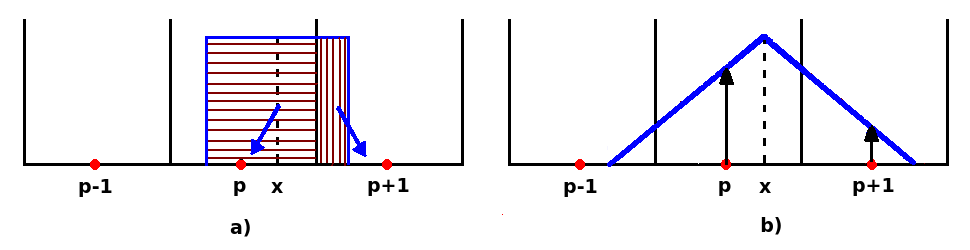
\includegraphics[width=0.8\textwidth]{Images/chapter3/CIC.png}
       \caption{\small Left: CIC cloud shape function and the intersection
       between the cell centered in the particle with the cells provides the contribution of
       the mass to every cell. Right: it shows a ''triangle''	 function that is evaluated
       in every grid point to find the charge contribution to the cell. 
      $x$ is the position of the particle and the indexes $p-1$, $p$ and $p+1$ are contiguous cells.}
       \label{CIC}
 \end{figure}
%**********************************************************************************************************************

\item \textbf{ Triangular shaped cloud (TSC): } This scheme is as the two previously presented but the cloud
shape and window function change. As it happens with CIC, TSC contributes to different
cells, not only the one where it falls in. Both interpretations are shown in the figure \ref{TSC}.
Next the expression to calculate the mass contribution to a specific cell is given by,

\begin{eqnarray*}
 W_{TSC}(x)  &=& \frac{1}{H}\Lambda \left( \frac{x}{H} \right)*\Pi \left(\frac{x}{H}\right) \\ 
&  = &\frac{1}{H}\Pi\left(\frac{x}{H}\right)*S\left(\frac{x}{H}\right) .
\end{eqnarray*}

The Fourier transform of the window function is, 

\[ W_{TSC}(k)= sinc^3\left(\frac{\pi k}{2k_N} \right),\]

hence, the Fourier transform of the TSC window function is the cubic of the Fourier 
transform of the NGP window function \cite{hockney}. 

\end{enumerate}

%**********************************************************************************************************************
\begin{figure}[htbp]
       \centering
               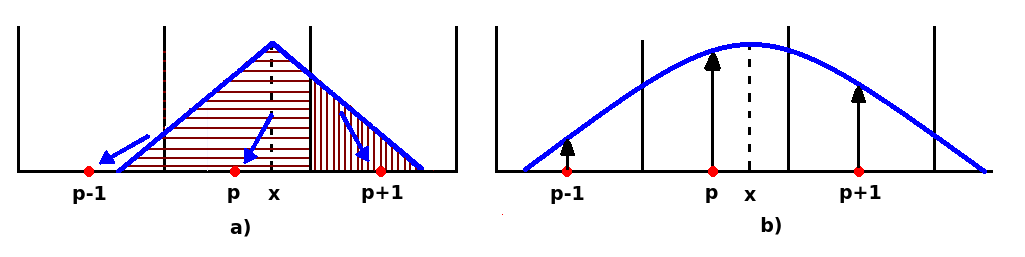
\includegraphics[width=0.8\textwidth]{Images/chapter3/TSC.png}
       \caption{\small Left: it shows the cloud shape function, a ''triangle'' function
       and the overlap with the cells provides the value of the charge assigned to every cell. 
       Right: it shows the window function interpretation, where the particle carries
       with a function that evaluated in every grid point gives the contribution to the specific cell. 
       $x$ is the position of the particle and the indexes $p-1$, $p$ and $p+1$ are contiguous cells.}
       \label{TSC}
 \end{figure}
%**********************************************************************************************************************


Hence, each successively higher order assignment function is obtained by convolving the previous
assignment function with $\frac{1}{H}\Pi\left(\frac{x}{H}\right)$. 

From a one dimensional window function can be obtained the three dimensional one, simply as
the multiplication of the three one dimensional ones. This last asseveration is valid due to 
the grid used is regular. 

Thus, for every cell contained in the cosmological box a value of the convolved density 
field is calculated using a specific mass assignment scheme. 

%&&&&&&&&&&&&&&&&&&&&&&&&&&&&&&&&&&&&&&&&&&&&&&&&&&&&&&&&&&&&&&&&&&&&&&&&&&&&&&&&&&&&&&&&&&&&&&&&&&&&&&&&&&&&&&&&&&&&&&
\section{ Power spectrum in cosmological simulations }
%&&&&&&&&&&&&&&&&&&&&&&&&&&&&&&&&&&&&&&&&&&&&&&&&&&&&&&&&&&&&&&&&&&&&&&&&&&&&&&&&&&&&&&&&&&&&&&&&&&&&&&&&&&&&&&&&&&&&&&


The density perturbations of the ensemble, convolved density field for every cell 
of the box, allow to calculate the power spectrum as shown in equation \ref{pk},
an esemble average for every mode $\kappa$. Since this is a statistical measure in
the Fourier space let us see the Fourier transform in more detail \cite{Mont}.

\subsection{Fourier transform}

The fourier transform is defined for this work with the next convention:

\begin{equation}
F(\boldsymbol{\kappa}) = \int_{-\infty}^{\infty} d^3 x f(\textbf{x})e^{-i \boldsymbol{\kappa}\cdot\boldsymbol{x}	},
\label{FT}
\end{equation}

with $\kappa$ being the wave number vector. The inverse fourier transform as:

\begin{equation}
f( \boldsymbol{x}) = \int_{-\infty}^{\infty} \frac{d^3 \kappa}{(2\pi)^3}  F(\boldsymbol{\kappa})e^{i \boldsymbol{\kappa}\cdot\bf{x}	}.
\label{IFT}
\end{equation}

The convolution of the functions $g(\bf{x})$ and $f(\bf{x})$ is defined as follows:

\[h(\bf{x}) = |g*f|(\bf{x})\equiv \int_{-\infty}^{\infty} g(\bf{x}')f(\bf{x} - \bf{x}') d^3 x' , \]

but the Fourier transform of $h(\bf{x})$ is: 

\[H(\boldsymbol{\kappa}) = G(\boldsymbol{\kappa}) F(\boldsymbol{\kappa}),  \]

this is known as the convolution theorem \cite{Djeong}. It is used in our work since the fourier 
transform of the window function convolved with the density field (equation \ref{df_conv})
allow us to obtain the real density field. From equation \ref{df_four}, 

\[\delta(\textbf{k}) = \delta^s(\textbf{k})/W(\textbf{k}).\]

In the situation we are dealing with, the function $F(\boldsymbol{\kappa})$ is only
sampled at evenly spaced intervals ($N^3$ frequencies totally) since we only 
know $f(\textbf{x})$ in $N^3$ points

\begin{eqnarray*}
F(\boldsymbol{\kappa}) =\left\{ \begin{array}{cl}
F(\kappa_F\boldsymbol{n}_\kappa) \hspace{1em} & \boldsymbol{n}_\kappa = (i,j,k) \in Z^3\\
0 \hspace{1em} & \mathrm{otherwise,} \\
\end{array}\right.
\end{eqnarray*} 

where $\kappa_F=2\pi/L$ is the fundamental frequency \cite{Djeong}.

Due to the functions are only sampled in specific points, the integrals defined in 
equations \ref{FT} and \ref{IFT} can be approximated to the discrete Fourier transform. 
Let us express them in terms of the density fluctuations in real and Fourier space 
because they are the ones of interest for our work: 

\begin{eqnarray*}
\delta(\boldsymbol{\kappa}_p) = H^3 \sum_{n_p} \delta(\boldsymbol{r}_p) e^{-i\boldsymbol{\kappa}_p\cdot \boldsymbol{x}_p}, \\
\delta(\boldsymbol{r}_p) = \frac{1}{L^3}\sum_{\boldsymbol{k}_p} \delta(\boldsymbol{\kappa}_p) e^{i\boldsymbol{\kappa}_p\cdot \boldsymbol{x_p}}, 
\end{eqnarray*} 

where $H = L/N$ is the separation of the grid in the real space, 
$\boldsymbol{\kappa}_p = k_F \textbf{n}_p$ and $ \boldsymbol{n}_p = (i,j,k)$ with each index
varying from $-N/2 \leq i,j,k \leq N/2$ . The function $\delta(\boldsymbol{r}_p)$  is sampled 
in the points $\boldsymbol{r}_p$ and $\delta(\boldsymbol{\kappa}_p)$ in the points 
$\boldsymbol{\kappa}_p$. Therefore, the Fourier space is divided into small cells, N cubes of size 
$\kappa_g = 2\pi/H$ per dimension as it was done for the simulation. 

Furthermore, the extreme values for $\boldsymbol{n}_p$ correspond to Nyquist critical 
frequency: 

\[\kappa_N = \pi\frac{N}{L} = \frac{\pi}{H}, \]

so $-\kappa_N < k < \kappa_N $. A phenomenon called aliasing appears when a continuous 
function is sampled and is not bandwidth limited to a frequency smaller than $\kappa_N$. 
It consists in a folding over or aliasing of the frequencies that fall outside the range
as shown in figure \ref{alias}. 

%**********************************************************************************************************************
\begin{figure}[htbp]
       \centering
               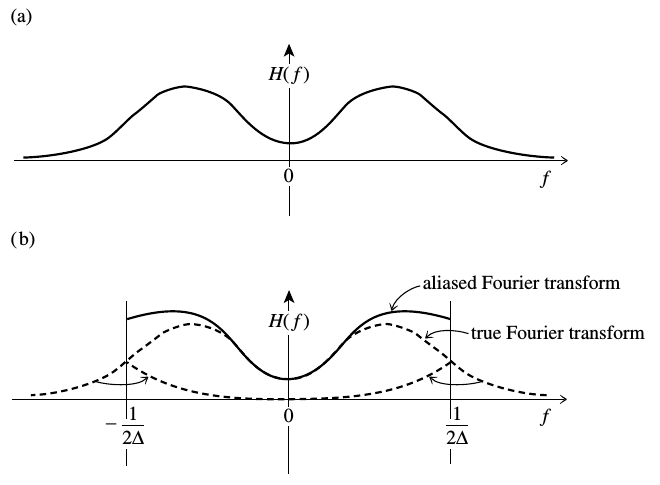
\includegraphics[width=0.8\textwidth]{Images/chapter3/aliasing.png}
       \caption{\small Aliasing effect for $H(f)$ sampled with a space interval $\Delta$.
       Frequencies outside the frequency range are included into the range because
       of the discrete sampling of the function. Figure taken from \cite{Press}.}
       \label{alias}
 \end{figure}
%**********************************************************************************************************************

To perform the discrete Fourier transform of the sampled density field was used the free 
library FFTW, where a fast Fourier discrete transformation (FFT) is implemented.
Because of algorithmic details of the FFT the fourier coefficients are ordered in the
following manner

\begin{eqnarray*}
\kappa_l(i) =\left\{ \begin{array}{cl}
\frac{2\pi}{L}i \hspace{1em} & \mathrm{if} \hspace{1em} i = 0,\dots ,\frac{N}{2}\\
\frac{2\pi}{L}(-N+i) \hspace{1em} & \mathrm{if} \hspace{1em} i = \frac{N}{2}+1,\dots ,N-1 ,\\
\end{array}\right.
\end{eqnarray*} 


where the subindex $l$ stands for $x,y$ or $z$ coordinate. 
The library has different routines, one is a complex to complex function, this is, perfoms a 
Fourier transformation of a sampled complex function. Other one, named real to complex routine, 
takes the real samples of a function to find the Fourier transformation. The last one 
uses the Hermitian condition that allows to improve the calculation in speed and memory 
usage \cite{Jing},

\[\delta_\kappa(-\textbf{n}_\kappa) = \delta_\kappa^*(\textbf{n}_\kappa),\]

where the superscript $*$ denotes complex conjugate. In both cases a normalization 
must be taken into consideration, this can be noticed in the relation between the transformed 
density field obtained with FFTW and the sampled space density field, 

\[\delta^{FFTW}(\textbf{n}_k) = \sum_{r_p} \delta(\textbf{r}_p)e^{-i\boldsymbol{\kappa}_p\cdot \boldsymbol{r}_p} = \frac{\delta(\boldsymbol{\kappa}_p)}{H^3},\]

with the last expression and the definition of PS given in equation \ref{pk}, the power
spectrum from FFTW is given by \cite{Djeong},

\begin{equation}
P(\kappa_F n_1) = \frac{H^6 k^3_F}{(2\pi)^3}\langle\delta^{FFTW}(\mbox{\boldmath$n$}_1\delta^{FFTW}(-\mbox{\boldmath$n$}_1)\rangle = \frac{V}{N^6}\langle|\delta^{FFTW}(\mbox{\boldmath$n$}_1)|^2\rangle ,
\end{equation} 

this is the power spectrum estimator that is used throughout this work. 

\subsection{PS calculation}

To calculate the power spectrum, the next steps are followed

\begin{enumerate}

\item[1)] From a cosmological box of size $L$, a grid with $N^3$ subdivisions is performed
creating cells of volume $H^3$. 

\item[2)] The sampled space density field is created using a specific window function,
mass of particles are assigned to the grid. 

\item[3)] With FFTW software, the FT of the sampled space density field is calculated.

\item[4)] To deconvolve and eliminate the aliasing effect $P(\boldsymbol{\kappa})\equiv |\delta(\kappa)|^2$ is divided by the next window function, at each grid point or equivalently each cell,

\[ W(\boldsymbol{\kappa}) = \prod^{3}_{i=1}\left[ 1 - \frac{2}{3}\sin^2\left(\frac{\pi\kappa_i}{2\kappa_N}\right) \right] ,\]

where $\boldsymbol{\kappa} = (\kappa_x,\kappa_y,\kappa_z)$ as proposed in \cite{Jeong}.  

\item[5)] The amount $P(\kappa)$ is calculated taking the spherical average of 
$P(\boldsymbol{\kappa})$ corrected inside the shell 
$\kappa -\Delta\kappa/2	< |\boldsymbol{\kappa}|<\kappa +\Delta\kappa/2$.

\end{enumerate}


%&&&&&&&&&&&&&&&&&&&&&&&&&&&&&&&&&&&&&&&&&&&&&&&&&&&&&&&&&&&&&&&&&&&&&&&&&&&&&&&&&&&&&&&&&&&&&&&&&&&&&&&&&&&&&&&&&&&&&&
\section{ Correlation functions in cosmological simulations }
\label{STM}
%&&&&&&&&&&&&&&&&&&&&&&&&&&&&&&&&&&&&&&&&&&&&&&&&&&&&&&&&&&&&&&&&&&&&&&&&&&&&&&&&&&&&&&&&&&&&&&&&&&&&&&&&&&&&&&&&&&&&&&


In practice, to calculate in a cosmological simulation the correlation function 
a at distance $r$, it has to be performed an average of the number of neighbours per 
particle at a given scale or the binned comoving separation. In this direction 
correlation function estimators can be used, one of the most basic ones is shown below. 
Two catalogues are considered for this estimator, one is the properties of the particles 
of the box, data-data catalogue (DD) and the second one is generated 
randomly with at least the same number of particles and the same size of the box, 
random-random catalogue (RR). The DD catalogue should have regions with more or
less clustering than a homogeneous distribution, this is precisely the RR catalogue role, 
a way to measure how much the DD catalogue deviates from the homogenous distribution \cite{CF_theor}. 

From this estimator is easier to notice that $\xi(r)$ is a measure of 
excess or deficiency of clustering at $r$ making it more intuitive, 

\[1+\xi(r)= \f{\eta_{DD}(r)}{\eta_{RR}(r)} ,\]

here $\eta_{RR}(r)$ is the number of pairs of particles at a distance $r$ in the catalogue DD 
and $\eta_{RR}(r)$ is the number of pairs of particles at a distance $r$ in the catalogue RR. 

Other common estimators also need an additional catalogue, the data-random, where the
pair of particles would not only include the DD or RR but a mixed catalogue containing 
both arrays, making more robust the estimator proposed \cite{Est_CF}:

\begin{eqnarray}
\mbox{Landy-Szalay Estimator}\hspace{0.5cm} \xi_{LS}(r)&=& 1+\frac{DD(r)}{RR(r)}\left(\frac{N_R}{N}\right)^2-2\f{DR(r)}{RR(r)}\left(\frac{N_R}{N}\right) , \nonumber \\
\mbox{Hamilton Estimator}  \hspace{0.5cm} \xi_{HAM}(r)&=&\frac{DD(r)RR(r)}{DR(r)^2}-1 , \nonumber 
\end{eqnarray}

where $N_R$ is the number of points of the RR catalogue and $N$ of the DD catalogue.

\subsection{Correlation function calculation}

To calculate the correlation function the Landy-Szalay estimator is used, the next
rough steps are followed to calculate it

\begin{enumerate}

\item[1)] A catalogue of $N_R$ particles is generated randomly in a cubic box of size L.

\item[2)] For a bin around $r$ the magnitude of the distances between DD, RR and DR
particles are found, that way, pairs of galaxies that are at a distance $r$ for every 
catalogue are obtained. Finally, using Landy-Szalay estimator the correlation function 
is calculated for each radial bin. 

\end{enumerate}